\documentclass[11pt,a4paper]{article}

\usepackage[utf8]{inputenc}
\usepackage[T1]{fontenc}
\usepackage[margin=1in]{geometry}
\usepackage{amsmath,amssymb,amsthm}
\usepackage{booktabs}
\usepackage{tabularx}
\usepackage{graphicx}
\usepackage{fancyhdr}
\usepackage{hyperref}
\hypersetup{colorlinks=true,linkcolor=blue,urlcolor=cyan,citecolor=blue}

\pagestyle{fancy}
\fancyhf{}
\fancyfoot[L]{\footnotesize\color{gray}Mahadeva, \emph{Supply restrictions: where employment falls, and why}. Working note v1.0, September 2026.}
\fancyfoot[R]{\footnotesize\color{gray}\thepage}
\renewcommand{\headrulewidth}{0pt}
\renewcommand{\footrulewidth}{0.2pt}
\usepackage{xcolor}

\setlength{\parskip}{0.6em}
\setlength{\parindent}{0pt}

\title{\textbf{Supply restrictions:\\where employment falls, and why}}
\author{Lavan Mahadeva}
\date{\today}

\begin{document}
\maketitle
\thispagestyle{fancy}

\begin{center}
\begin{minipage}{0.92\textwidth}
\small
\textbf{Abstract.} Restricting the supply of one input at the top of a production chain reduces employment at every stage of it. This note sets out a chain of $S$ producing stages and a household, with the cost share, the elasticity of substitution and the elasticity of supply of own inputs all free to differ between stages, and reduces it to $S$ linear equations in $S$ unknowns. Employment at each stage then splits into three terms: employment per unit of output rises, output falls because the stages downstream buy less, and output falls because households buy less. Calibrated to the American H-2B visa cap and the USDA food dollar, a 20 percent rise in the price of seasonal labour reduces employment by 2.21 percent at harvesting, 1.03 percent at processing and 0.32 percent at retail; where pay follows the cost of living and the restricted input is used throughout the economy, every stage loses over five percent.
\end{minipage}
\end{center}

\medskip

\begin{center}
\begin{minipage}{0.92\textwidth}
\footnotesize
\textbf{Cite as:} Mahadeva, L. (2026). \emph{Supply restrictions: where employment falls, and why.} Working note v1.0. DOI: \href{https://doi.org/10.5281/zenodo.22836881}{10.5281/zenodo.22836881}.

\textbf{Code and verification:} every number in this note is computed rather than typed. The model, and a script that recomputes all 66 printed figures and checks them against the text, are archived with this note.
\end{minipage}
\end{center}

\bigskip

Sections~\ref{sec:intro} to~\ref{sec:ignore} are plain English and contain the argument. Section~\ref{sec:model} sets out the model, with every parameter free to differ between stages. Section~\ref{sec:example} puts numbers in. Section~\ref{sec:obj} answers the objections and lists what is weak.

\section{Introduction}
\label{sec:intro}

Michael Clemens and Ethan Lewis published an interesting paper on the impact of restrictions on seasonal immigrant labour on the employment of other workers, which is summarised here \href{https://cepr.org/voxeu/columns/restricting-hiring-low-skill-immigrants-hurts-firms-and-does-not-benefit-native-born}{VoxEU}.

I wrote this note because the policy they analysed seemed to me to be symptomatic of our times. Our real income is under stress as growth rates have slowed and even stalled, and debt levels seem unaffordable. Yet, we still face further threats to our standard of living and the public continue to clamour for governments to help; ``Do something!'' Politicians, well aware of the power of social media to cost an election, compete to respond with solutions that treat an unpopular symptom. Examples would be restrictions on hiring immigrants; restricting external inputs with tariffs or quotas; capping prices; protecting wages and employment. But the marketing of these policies often brushes over the fact that modern economies work in chains with specialisms. Even in the case of farming, production runs through several stages: someone harvests, someone processes and packs, someone transports, someone sells, households buy. When the supply of an input in a chain is restricted, and further layers of protection are added, the impact can easily be larger than what we can generously say was intended.

In 1973, Horst Rittel and Melvin Webber, a design theorist and an urban planner at the University of California, Berkeley, set out ten features that make a problem ``wicked''. Its definition is contested, there is no objective ``stopping rule'', answers are good or bad rather than true or false, and which explanation you accept depends on your own view of the world. Their warning was against treating such problems as tame. Their reason is the one this note is about — every wicked problem can be considered a symptom of another problem, and interventions treat the symptom at one point in the chain without making the extra effort to explain to the public that it is not that easy.

\section{The Clemens and Lewis study}
\label{sec:study}

The policy Michael Clemens and Ethan Lewis analysed restricted immigrant labour, with the stated aim of protecting the pay
and jobs of American workers. The H-2B visa covers seasonal work outside agriculture: landscaping, seafood processing, forestry, hospitality. Ninety-eight percent of the jobs need no high school education, and employers ask for 1.2 months of experience on average.

Congress capped the programme at 66,000 visas a year in the Immigration Act of 1990, split into 33,000 for each half of the fiscal year. Michael Clemens asked Bruce Morrison, who chaired the House Immigration Subcommittee and helped write the Act, where the number came from. The drafters took the 22,115 visas issued the previous year, tripled it, and assumed a ceiling that high would never be reached. Employers have asked for more every year since. For the second half of 2022 they asked for 136,555 workers against 33,000 places. For 2026 the government issued the statutory 66,000 plus a supplement of 64,716, the legal maximum, and still ran out.

The queue is what makes the cap worth testing, because the government then had to ration it at random. After so many petitions arrived at once in 2019 that the Labor Department's server crashed, it began giving each petition a random letter, A to E in 2021 and A to G in 2022, and processing the A petitions first. A firm drawing an A gets almost all the workers it asks for. A firm drawing a late letter gets few. Which letter a firm draws has nothing to do with the firm.

Clemens and Lewis surveyed 472 firms that entered the 2021 and 2022 draws, and registered their hypotheses before any responses arrived, which stops a researcher choosing the results they like after seeing the data. Losing the draw cut a firm's employment of these workers by about half.

Four of their results matter for what follows.

\textbf{The firms that lost got smaller.} Revenue rose with an elasticity of 0.20
to 0.22 in H-2B employment, so halving that employment cut revenue by about 12
percent. This fall in output is what the rest of this piece is about.

\textbf{The jobs did not move to American workers.} Employment of low-skill
American workers at the losing firms did not rise. Across all firms the effect of
foreign hiring on American employment was zero or positive, and in a rural sample
specified in advance it was positive and significant, at 0.61: one percent more
H-2B workers came with just over half a percent more American workers.

\textbf{The two kinds of worker are poor substitutes.} Clemens and Lewis estimate
the elasticity of substitution between H-2B and American workers at 0.8 to 2.2,
which is the percentage change in the ratio of the two a firm employs for each one
percent change in their relative wage. Related studies of immigrants in low-skill
work usually find 4 to 10. A lot of what follows depends on this understanding.

\textbf{Machinery did not replace the workers either.} Investment in equipment,
vehicles and buildings rose with an elasticity of 1.5 to 2.1 in H-2B employment,
so restricting the labour reduced the investment. Equipment and these workers are
used together, which is why I treat a stage's own inputs as labour and equipment
together rather than as two separate things.

One further result is worth noting and setting aside for now. The profit rate rose with
an elasticity of 0.15, which suggests these firms hold some surplus. I assume
abnormal profit is zero or constant, and return to it later.

Hein de Haas makes a general point in his book \emph{How Migration Really Works} (2023).
The demand for immigrant workers is structural, because the jobs need someone
physically present, so restricting the supply does not remove the demand. Two of
the twenty-two myths he discusses are that border restrictions reduce immigration, and that
immigrants take native jobs and hold down wages. Clemens and Lewis supply
firm-level evidence on both.

What the restriction changes is the size of the firm. Lewis summarised it: ``If you don't allow firms to hire immigrant workers, they
just become smaller firms. They are not replaced with US workers. Instead, the output of the firm shrinks, and there are fewer total workers.''


\section{What simplistic policies around supply restrictions often ignore}
\label{sec:ignore}

Simplistic marketing of supply restriction policies typically ignores three things.
\begin{itemize}\itemsep2pt
\item \emph{That the restricted input may not be easily substitutable.} It is too easy to assume that low-wage labour can be swapped for other inputs just because it is paid less. But comparative advantage may be at work, allocating the best mix of work to the factors available and reversing that can be costly. Clemens and Lewis measure an elasticity of substitution between migrant and US workers of 0.8 to 2.2. That is above one, so the two are substitutes, but it is well below the 4 to 10 that related studies of immigrants in low-skill work typically find. On their estimate, foreign and US hires in these low-skill jobs are at least as different to a firm as college and non-college workers are. They also rule out that the firms which lost the draw substituted machinery for workers. And native hiring did not rise when migrant hiring was cut, and may have fallen slightly. Section~\ref{sec:caveats} shows the arithmetic. (What reduced employment was the fall in the firm's scale, not a switch between the two kinds of worker, which I explain below). In 1993, Michael Kremer described an extreme case of this, about a humble piece of rubber. The space shuttle Challenger had thousands of components. It exploded in 1986 because one of them, an O-ring seal, failed in the cold. Kremer's model treats production as a set of tasks whose qualities multiply rather than add, so the value of doing any one task well rises with how well the others are done. Restrict one input in a chain like that and you lose more than that input: you reduce what the inputs working alongside it are worth. Another example of brushing aside this problem is assuming that green technologies are plug-and-play substitutes for fossil fuel ones.

\item \emph{The tension that arises if productivity falls.} When an important complementary input is restricted, the productivity of other inputs falls. This puts pressure on the pay of the other workers, and then those workers could resist wage cuts, making it even more likely that firms shrink. No one wants the pain but how you avoid it can make it larger. Bruno and Sachs called the general version of this real wage resistance, and used it to explain why the oil shocks of the 1970s led to much higher unemployment in some economies than in others, and attributed the difference to how far real wages adjusted.

\item \emph{That consumers buy less of more expensive items.} A stage that cannot let the price it pays fall will try to pass the cost on to the stage that buys from it, and if it cannot do that either, it produces less. Of course, this may be the whole intent of the policy: we do not like this industry, or it is no longer sustainable, so let it shrink. But policies are rarely presented in these terms. The cap was justified as protecting American jobs and pay. And on either justification the falls in demand, output and employment along the chain are a cost, and they should be measured.
\end{itemize}

How might taking account of these complexities matter? To answer this, I built a model to illustrate the scale using Clemens and Lewis's example.

I set up a chain of three producing stages — harvesting, processing and packing, retail and food service — selling to households. Farms receive 11.8 cents of every dollar Americans spend on domestically produced food, which the USDA food dollar series measures. I matched that with cost shares of 0.40, 0.60 and 0.50 at the three stages, which multiply to 0.120. That 11.8 cents is what farms receive in total, not what they pay seasonal workers. I used it anyway, which overstates the share: for visa labour alone it is perhaps 0.01 to 0.03, and if so, every figure below falls in proportion (more on this later). I assumed each stage switches away from a dearer input slowly, by 0.15, 0.30 and 0.45 percent for each percent of change in relative prices, rising downstream. Those are well below the 0.8 to 2.2 that Clemens and Lewis measure, because one firm can hire another firm's workers while the whole sector cannot, and because I ruled out buying the intermediate input abroad. Food at home and at restaurants is about a seventh of total household consumption, which puts the price elasticity of food demand at 0.5 and gives food a weight of 0.15 in the index that pay follows. Seasonal work is the kind people move in and out of, so I assumed each stage can hire as much of its own inputs as it wants at the going rate: pay follows the cost of living, and employment takes the adjustment. The restriction itself is a 20 percent rise in the price of seasonal labour, which I guessed or assumed.

Employment falls at all three stages, and falls most in percentage terms at the stage the cap applies to: harvesting loses 2.21 percent, processing 1.03 percent and retail 0.32 percent. Output falls by more at each of them, by 3.38, 2.44 and 1.38 percent, because every stage employs more of its own inputs per unit of what it makes — between 1.06 and 1.41 percent more — which recovers part of the fall. No pay falls anywhere. All three factor prices rise by 0.41 percent, the rise in the cost of living, against selling prices that rise by 8.25 percent at the farm gate, 5.12 percent at wholesale and 2.76 percent on the shelf. Indexing pay to the cost of living takes the share of the original rise that reaches the shelf from 12 percent to 13.8 percent, so households buy 1.38 percent less rather than 1.20 percent less. That amplification is small, because food is about a seventh of total household consumption and the index barely moves.

For an input used throughout the economy the same mechanism would be far larger.

\section{The model}
\label{sec:model}

Production has S stages and the household is stage S+1. Stage s combines the output of the stage before it with its own inputs:

\begin{equation}
Y_s = F_s(Y_{s-1}, L_s), \qquad s = 1, \dots, S+1 .
\end{equation}

$L_s$ is the labour, plant and machinery hired at stage s. I call changes in $L_s$ changes in employment throughout, which is shorthand: it covers equipment as well as workers. For the household, $Y_S$ is the good it buys and $L_{S+1}$ is everything else it spends money on.

$Y_0 = X$ is the restricted input and I assume it is in the first stage. We can work through an example where the restriction is in the middle of a chain, but I will save that for a rainy day. $P_s$ is the price of stage-s output, with $P_0 = P_X$. $W_s$ is the price stage $s$ pays for its own inputs: in this case, wages and equipment rents.

Stage numbers rise along the chain. Stage $s$ buys from stage $s-1$ and sells to stage $s+1$, so a higher number means further from the restricted input and closer to the household. I say \emph{upstream of k} for stages numbered below k, which supply it, and \emph{downstream of k} for stages numbered above k, which buy from it.

Each producing stage sells at a price equal to its cost per unit, so abnormal profit is zero or constant. Each buys its intermediate input only from the stage immediately upstream of it, and no stage can import a substitute for what the restricted chain makes. So $\sigma_s$ is substitution between the domestic intermediate input and the stage's own labour and equipment, and nothing else. That is why the elasticities of substitution used throughout are low: a sector cannot do what one firm in it can. Lower case letters are percentage changes, so $p_s$ is the percentage change in $P_s$.

\subsection{The core logic}
\label{sec:core}

A firm at stage $s$ hires its own inputs up to the point where the price it pays for them equals the revenue the last unit brings in:

\begin{equation}
W_s = P_s \cdot \frac{\partial F_s}{\partial L_s} .
\end{equation}

The right-hand side is the price of output times the extra output the last unit of input produces. Economists call it the marginal revenue product. This condition holds for the same reason at every stage: if the price paid were lower than that the firm would hire more, and if higher it would hire fewer.

What happens if we restrict the supply of the input at the top of the chain? Its price rises, so the price of stage-1 output rises, and so on down. At any stage whose output price has risen, the right-hand side has risen, so the condition requires either that $W_s$ rises by the same percentage, or that the marginal product falls by the difference.

Written in percentage changes, and using the definition of the elasticity of substitution, the condition becomes

\begin{equation}
\underbrace{l_s - y_s}_{\text{employment per unit of output}} \;=\; \sigma_s \,(p_s - w_s) .
\end{equation}

$\sigma_s$ is the elasticity of substitution at stage s: the percentage change in the ratio of the two inputs the stage uses, for each one percent change in their relative price. It can be anything from zero, complements in strict fixed proportions, to positive infinity, perfect substitutes. The same first-order condition applied to the intermediate input gives

\begin{equation}
\underbrace{y_{s-1} - y_s}_{\text{purchases from upstream, per unit of output}} \;=\; \sigma_s \,(p_s - p_{s-1}) .
\end{equation}

We can also combine the two as
\begin{equation}
\underbrace{l_s - y_{s-1}}_{\text{own inputs, per unit of what it buys from upstream}} \;=\; \sigma_s \,(p_{s-1} - w_s) .
\end{equation}

All of this goes to say that when one input gets dearer relative to another, the firm uses less of the dearer one, by $\sigma_s$ percent for each percent of relative price change.

The household is stage $S+1$. Its real spending is assumed fixed, so $y_{S+1}$ = 0, and the price of everything else it buys is the numeraire, so $w_{S+1}$ = 0. Substituting gives the demand curve:

\begin{equation}
y_S = -\eta \, p_S, \qquad \eta = \sigma_{S+1}(1-\theta_{S+1}) ,
\end{equation}

where $\theta_{S+1}$ is the share of the household budget spent on the good. So the price elasticity of final demand is the household's elasticity of substitution, multiplied by the share of its budget spent on everything else. A good that takes a small share of the budget has a demand elasticity close to the household's full elasticity of substitution. A good that takes the whole budget has an inelastic demand, because there is nothing left to switch to. This is core applied microeconomics: Alfred Marshall made the same point about inputs in 1890 in one of the first economic textbooks, in the chapter on joint and composite demand.

\subsection{How far factor prices are allowed to change matters}
\label{sec:factor}

Two things decide how far the price a stage pays for its own inputs moves: what that pay is tied to, and how easily more of the input can be had.

Pay follows the cost of living. Write $\pi$ for the percentage rise in the consumer price index. Only part of what a household buys contains the restricted input, so

\begin{equation}
\pi \;=\; \lambda \, p_S , \qquad \lambda \in [0,1] .
\end{equation}

$\lambda$ is the share of the consumer basket whose price moves with the restricted input, multiplied by how fully pay is indexed to the index. Only the product of the two can be identified, so it is one parameter. For a single sector $\lambda$ is near that sector's budget share. For an input used throughout the economy it approaches one. Energy is about 6 percent of American household consumption and an input to most of the rest, so its $\lambda$ is well above that; getting it needs an input-output calculation rather than a reading off the published weights.

More of an input can usually be had only at a higher price. How much more is the elasticity of supply of stage-$s$ own inputs, $\varepsilon_s$, and it is the second and last parameter:

\begin{equation}
l_s \;=\; \varepsilon_s \,(w_s - \pi) , \qquad \varepsilon_s \in [0, \infty] .
\end{equation}

More of the input is offered when the pay it earns rises faster than the cost of living, and by $\varepsilon_s$ percent for each percent it does.

\begin{itemize}\itemsep2pt
\item $\varepsilon_s = \infty$. Supply is perfectly elastic. Pay tracks the cost of living and nothing else, and the whole adjustment falls on employment.
\item $\varepsilon_s$ = 0. Supply is fixed. Employment cannot move, so pay takes the whole adjustment and falls until every worker is still employed.
\item Between the two the adjustment is split between pay and jobs.
\end{itemize}

Wages always equal marginal revenue product. What $\lambda$ and $\varepsilon_s$ determine is whether wages or employment adjust.

So $\varepsilon_s$ sets a trade-off inside a stage, between the price paid for its own inputs and the quantity of them employed. A lower $\varepsilon_s$ reduces the fall in employment and increases the fall in pay. It cannot change the sign of either. The restriction imposes a cost on the stage whatever $\varepsilon_s$ is; what the value of $\varepsilon_s$ determines is whether the cost appears in pay or in jobs.
We can also define a useful variable $r_s$ which is how much more the price of the intermediate input the stage buys has risen than the price of the inputs it supplies itself.
\begin{equation}
r_s \;=\; p_{s-1} - w_s
\label{eq:rdef}
\end{equation}

Then the shift in the input mix called $\alpha_s$ is calculated as
\begin{equation}
\alpha_s  \;=\; d \ln \frac{L_s}{Y_{s-1}}=\sigma_s \, r_s  .
\end{equation}

One thing this specification does not capture is a minimum wage, or a union contract that ties pay to the employer's own selling price, in other words, it does not include a restriction on the product wage. What is here is more economy-wide behaviour and norms rather than firm-level agreements: workers defending what their pay buys, and unrestricted workers having outside options, with changes in employment possible.


\subsection{Solving the model}
\label{sec:solving}

The model reduces to $S$ linear equations in $S$ unknowns, one for each stage. This subsection writes them down and then recovers every other variable from the solution.

Once we solve for the $r_s$ across the whole chain, we can calculate $p_{s-1}$ and $w_s$ and every other variable.
\subsubsection*{The system}

Each stage's supply curve, $l_s = \varepsilon_s(w_s - \lambda p_S)$, is one equation. Substitute out every variable except $r$, and divide row $s$ by

\begin{equation}
c_s \;=\; \underbrace{\varepsilon_s(1-\lambda)}_{\text{its own inputs}} \;+\; \underbrace{\eta}_{\text{its buyers}} .
\end{equation}

$c_s$ is the total response of stage $s$ to the price it faces. The first part is how much more of its own inputs it can hire by paying more relative to the cost of living. The second is how much its buyers cut back when it charges more. What is left is

\begin{equation}
\tilde A\, r \;=\; p_0\, \mathbf{1} ,
\label{eq:system}
\end{equation}

\begin{center}
\small
\begin{tabular}{lll}
\toprule
\textbf{entry} & \textbf{value} & \textbf{what it measures} \\
\midrule
$\tilde A_{sm}$, $m < s$ & $1-\theta_m$ & what each upstream stage $m<s$ absorbs\\
$\tilde A_{ss}$ & $1 - \theta_s\,(d_s - \hat\sigma_s)$ & what the stage itself absorbs \\
$\tilde A_{sm}$, $m > s$ & $(1-\theta_m)\,(d_s - \hat\sigma_m)$ & what each downstream stage $m>s$ absorbs \\
\bottomrule
\end{tabular}
\end{center}

\begin{equation}
d_s \;=\; \frac{\eta - \lambda \varepsilon_s}{c_s} ,
\qquad
\hat\sigma_m \;=\; \frac{\sigma_m}{c_s} .
\end{equation}

So $r = \tilde A^{-1} p_0 \mathbf{1}$. $\tilde A$ is a general $S \times S$ matrix, and has to be inverted.

\subsubsection*{Reading the matrix}

The lower triangle contains no elasticity. It is $1 - \theta_m$, the share of a price rise that stage $m$ absorbs instead of passing on. Everything upstream of stage $s$ enters through cost shares alone.

The right-hand side is the same number in every row. Row $s$ states that the whole rise $p_0$ is accounted for in three ways: what the stages upstream absorb, what stage $s$ does itself, and what the stages downstream send back.

The diagonal and the upper triangle both contain $d_s - \hat\sigma_m$, with the sign reversed and a different weight: $\theta_s$ on the stage itself, $1-\theta_m$ on each stage downstream.

We can move the lower triangle to the right-hand side:

\begin{equation}
\resizebox{\textwidth}{!}{$\displaystyle
\underbrace{\big[1 - \theta_s(d_s - \hat\sigma_s)\big] r_s
\;+\; \sum_{m>s} (1-\theta_m)\,(d_s - \hat\sigma_m)\, r_m}_{\text{stage } s \text{ and the stages downstream of it}}
\;=\;
\underbrace{p_0 - \sum_{m<s}(1-\theta_m)\, r_m}_{=\; p_{s-1}, \text{ the price entering stage } s}
$}
\end{equation}

Each row now states one thing: stage $s$ and the stages downstream of it respond to the price that enters stage $s$, and not to the price of the restricted input. In this form $\tilde A$ is upper triangular. That is a reorganisation and not a solution, because $p_{s-1}$ still depends on the $r_m$ upstream of $s$. What it does is identify the only route by which anything upstream matters: the single number $p_{s-1}$.



\subsubsection*{The example}

At the calibration of Section~\ref{sec:example}, $S = 3$ and supply is perfectly elastic. So $\hat\sigma_m = 0$ at every stage, which means the price path does not depend on how easily any stage substitutes; substitution decides quantities only. And $d_s = -\lambda/(1-\lambda) = -0.1765$. With $\theta = (0.40, 0.60, 0.50)$ the system is

\begin{equation}
\begin{pmatrix}
\phantom{0}1.0706 & -0.0706 & -0.0882 \\
\phantom{0}0.6000 & \phantom{-}1.1059 & -0.0882 \\
\phantom{0}0.6000 & \phantom{-}0.4000 & \phantom{-}1.0882
\end{pmatrix}
\begin{pmatrix} r_1 \\ r_2 \\ r_3 \end{pmatrix}
=
\begin{pmatrix} 0.20 \\ 0.20 \\ 0.20 \end{pmatrix} ,
\qquad
r = \begin{pmatrix} 0.1959 \\ 0.0783 \\ 0.0470 \end{pmatrix} .
\end{equation}

We have three equations, three unknowns, and one matrix inversion. Moving the lower triangle across gives the same three rows read the other way, each driven by the price that enters:

\begin{center}
\small
\begin{tabular}{lll}
\toprule
& \textbf{row} & \textbf{change in the price} \\
\midrule
$s=1$ & $1.0706\, r_1 - 0.0706\, r_2 - 0.0882\, r_3 = p_0$ & 20.000\% \\
$s=2$ & $1.1059\, r_2 - 0.0882\, r_3 = p_1$ & \phantom{0}8.249\% \\
$s=3$ & $1.0882\, r_3 = p_2$ & \phantom{0}5.115\% \\
\bottomrule
\end{tabular}
\end{center}

The off-diagonal entries are small here because $\lambda$ is small. Set $\lambda = 0$ and they vanish: each stage would be settled by the price entering it and by nothing else, and the chain would solve in one pass down.

\subsubsection*{Recovering the rest}

With $r$ in hand every other variable follows in order, and none of it is a further choice. Stage 0 is the restricted input and stage $S+1$ is the household.

\textbf{Prices along the chain.} Each stage cuts the price entering from upstream by $(1-\theta_s) r_s$:

\begin{equation}
p_s \;=\; p_{s-1} - (1-\theta_s)\, r_s , \qquad s = 1, \dots, S .
\end{equation}

So the price at any stage is the original rise minus what every stage upstream of it has already absorbed. That holds whatever the parameters are.

\textbf{Factor prices and the cost of living.}

\begin{equation}
w_s \;=\; p_{s-1} - r_s , \qquad \pi \;=\; \lambda\, p_S .
\end{equation}

The first is equation~(\ref{eq:rdef}) rearranged, and it adds no information of its own. It is where the wage comes from once $r$ is known. The supply curves are satisfied without being imposed again, because choosing $r$ to satisfy them is what equation~(\ref{eq:system}) did.

\textbf{The shift in the input mix.}

\begin{equation}
\alpha_s \;=\; \sigma_s\, r_s \quad (s = 1, \dots, S) ,
\qquad
\alpha_{S+1} \;=\; \sigma_{S+1}\, p_S .
\end{equation}

The household is included because it is stage $S+1$. The price it faces has risen by $p_S$ and the price of everything else it buys is the numeraire, so its own $r$ is $p_S$.

\textbf{Output, working back from the household.} Set $y_{S+1} = 0$ and

\begin{equation}
y_s \;=\; y_{s+1} - (1-\theta_{s+1})\, \alpha_{s+1} , \qquad s = S, S-1, \dots, 1 .
\end{equation}

At $s = S$ this returns the demand curve of Section~\ref{sec:core}, $y_S = -\eta\, p_S$ with $\eta = \sigma_{S+1}(1-\theta_{S+1})$. At each stage upstream of that it subtracts $(1-\theta_{s+1})\alpha_{s+1}$, the cut its own buyer has made per unit of what that buyer makes. Those cuts accumulate moving up the chain, so output falls further the nearer a stage is to the restriction.

\textbf{Employment.}

\begin{equation}
l_s \;=\; y_s + \theta_s\, \alpha_s .
\end{equation}

The stage shifts its input mix by $\alpha_s$, and the share $\theta_s$ of that shift is employing more of its own inputs per unit of what it makes. That part is positive. Output has fallen, so the other part is negative, and the sign of the total is ambiguous.

The two do not interact. In percentage changes they add. In levels they multiply, because employment equals employment per unit of output times output. So a fall in output does not make the change in the input mix smaller. It makes it worth less, because there is less output to apply it to.

Everything from here on is the same $l_s$ but rearranged for interpretation. Nothing further is solved.

\textbf{Employment as three terms.} Substitute the output line into the employment line:

\begin{equation}
\resizebox{\textwidth}{!}{$\displaystyle
l_k \;=\;
\underbrace{\theta_k \alpha_k}_{\text{employment per unit of output rises}}
\;\underbrace{-\;\sum_{j=k+1}^{S} (1-\theta_j)\,\alpha_j}_{\text{output falls: stages downstream buy less}}
\;\underbrace{-\;\eta \, p_S}_{\text{output falls: households buy less}}
$}
\end{equation}

Here, as in Section~\ref{sec:example}, the results are reported without $\varepsilon$ or $\lambda$, because neither appears. Those two set $r$, and once $r$ is known the split holds whatever pay is tied to. The last term contains no $k$, so that part of the fall in output is the same percentage at every stage in the chain, from the farm to the checkout, and no firm's decisions change it. The middle term is empty at the last producing stage, because no producing stage buys from it.

\textbf{The same employment as a recursion.} Start at the household and work upstream:

\begin{equation}
l_{S+1} = \theta_{S+1}\,\alpha_{S+1} ,
\qquad
l_k = l_{k+1} + \theta_k\,\alpha_k - \alpha_{k+1} .
\end{equation}

The first is the employment line itself at $s = S+1$, because $y_{S+1} = 0$. The household hires nobody, so $l_{S+1}$ is not employment: $L_{S+1}$ is everything else the household buys, and $l_{S+1}$ is the change in what it spends on that.

Your own shift in input mix is worth $\theta_k \alpha_k$ to you, only the fraction $\theta_k$ of it, because the rest of the shift is a cut in what you buy, which does nothing for your own employment. The next stage's shift costs you $\alpha_{k+1}$, all of it. The part it puts into its own inputs is its employment gain and not yours, and the part it takes out of purchases is taken out of your output. Both work against you.

So a stage gains a fraction of its own effort and loses the whole of its customer's. The fraction is its cost share. A stage that is a small part of its customer's costs keeps little of what it does and absorbs everything its customer does. Being a minor line item in someone else's cost base is not protection.

\textbf{The last producing stage, at any supply elasticity.} Employment there has a closed form:

\begin{equation}
l_S \;=\; p_S \,\big[\sigma_S (1-\lambda) - \eta\big] \, \frac{\varepsilon_S}{\varepsilon_S + \sigma_S} .
\label{eq:lastst}
\end{equation}

Employment at the last stage falls while $\sigma_S(1-\lambda) < \eta$ and rises above it. Two elasticities of substitution counteract each other. $\sigma_S$ is how readily the stage switches away from the input that has become dearer. $\eta$ is how readily its customers switch away from what it sells. The stage gains employment only if it can switch faster than its customers can.

When the restriction moves the price of this sector and nothing else, $\lambda$ equals the household's budget share $\theta_{S+1}$. Since $\eta = \sigma_{S+1}(1-\theta_{S+1})$, the budget share then cancels from both sides and the condition is $\sigma_S > \sigma_{S+1}$. The share does two jobs of equal size in opposite directions: a larger share defends pay more, which reduces the stage's substitution, and makes demand less elastic, which reduces the fall in output.

So a small budget share does not protect employment in the last stage, and plentiful substitutes for what the chain produces do not help it either. Both work the other way. Cutting the budget share from 0.60 to 0.05 takes it from $-$0.28 to $-$0.33 percent. Raising $\sigma_{S+1}$ from 0.2 to 2.0 on the calibration of Section~\ref{sec:example} takes retail employment from $+$0.59 percent to $-$3.64 percent as customers switch (from restaurant meals to home cooking). What does change the sign is the stage's own $\sigma_S$ and its ability to adapt its offering out of the restricted chain: at 0.45 retail loses 0.32 percent, at 0.59 it breaks even, and at 1.0 it gains 0.97 percent.

It is also useful to look at cost shares. Let $\theta_s$ be the share of stage-$s$ revenue paid out for the intermediate input, and multiply these shares along the chain:

\begin{equation}
\Omega_{f \to k} \;\equiv\; \prod_{m=f+1}^{k} \theta_m
\;=\; \prod_{m=f+1}^{k} \frac{P_{m-1}Y_{m-1}}{P_m Y_m}
\;=\; \frac{P_f Y_f}{P_k Y_k} .
\end{equation}

$\Omega$ from f to k is the cost share of stage-f output in the value of stage-k output. $\Omega$ from 0 to S is the value of the restricted input as a share of what final households spend.


\subsection{A special case}
\label{sec:special}


$\tilde A$ is lower triangular when $d_s - \hat\sigma_m = 0$ for every $m > s$, which happens when supply is perfectly elastic and $\lambda = 0$. Then the chain solves in two passes, one down and one back. Each parameter fills the upper triangle in its own way: a finite $\varepsilon_s$ through $\hat\sigma_m$, which is the stages downstream cutting their purchases, and $\lambda$ through $d_s$, which is their effect on the cost of living.

\begin{center}
\fbox{\begin{minipage}{0.94\textwidth}
\smallskip
When the supply of every stage's own inputs is perfectly elastic, every wage is the same number, $\lambda p_S$, and the system collapses:

\begin{equation}
p_s \;=\; \Omega_{0 \to s}\, p_0 \;+\; \lambda\, p_S\,(1 - \Omega_{0 \to s}) ,
\qquad
p_S \;=\; \frac{\Omega_{0 \to S}\, p_0}{1 - \lambda\,(1 - \Omega_{0 \to S})} .
\end{equation}

Each stage's price is a weighted average of two things: the price of the restricted input, and the cost of living. The weight is the cumulative cost share. A stage close to the restriction is mostly the first; a stage far from it is mostly the second.

The second expression is a multiplier. Write the effective cumulative share as

\begin{equation}
\tilde\Omega_{0 \to S} \;=\; \frac{\Omega_{0 \to S}}{1 - \lambda(1 - \Omega_{0 \to S})}
\;=\; \Omega_{0 \to S}\,\Big[\, 1 + \lambda(1-\Omega_{0 \to S}) + \lambda^2 (1-\Omega_{0 \to S})^2 + \dots \Big] .
\end{equation}

The price rise lifts the cost of living by $\lambda$ of it, which lifts every wage, which lifts prices again by the share that wages account for. Each round is $\lambda(1-\Omega)$ of the one before. That fraction is the leakage.
\smallskip
\end{minipage}}
\end{center}

What an input costs as a share of the final price can be estimated. How much of a rise in its price reaches the buyer also depends on how much of the rest of the basket moves with it, and on how many times round the chain that feeds back.

\begin{figure}[htbp]
\centering
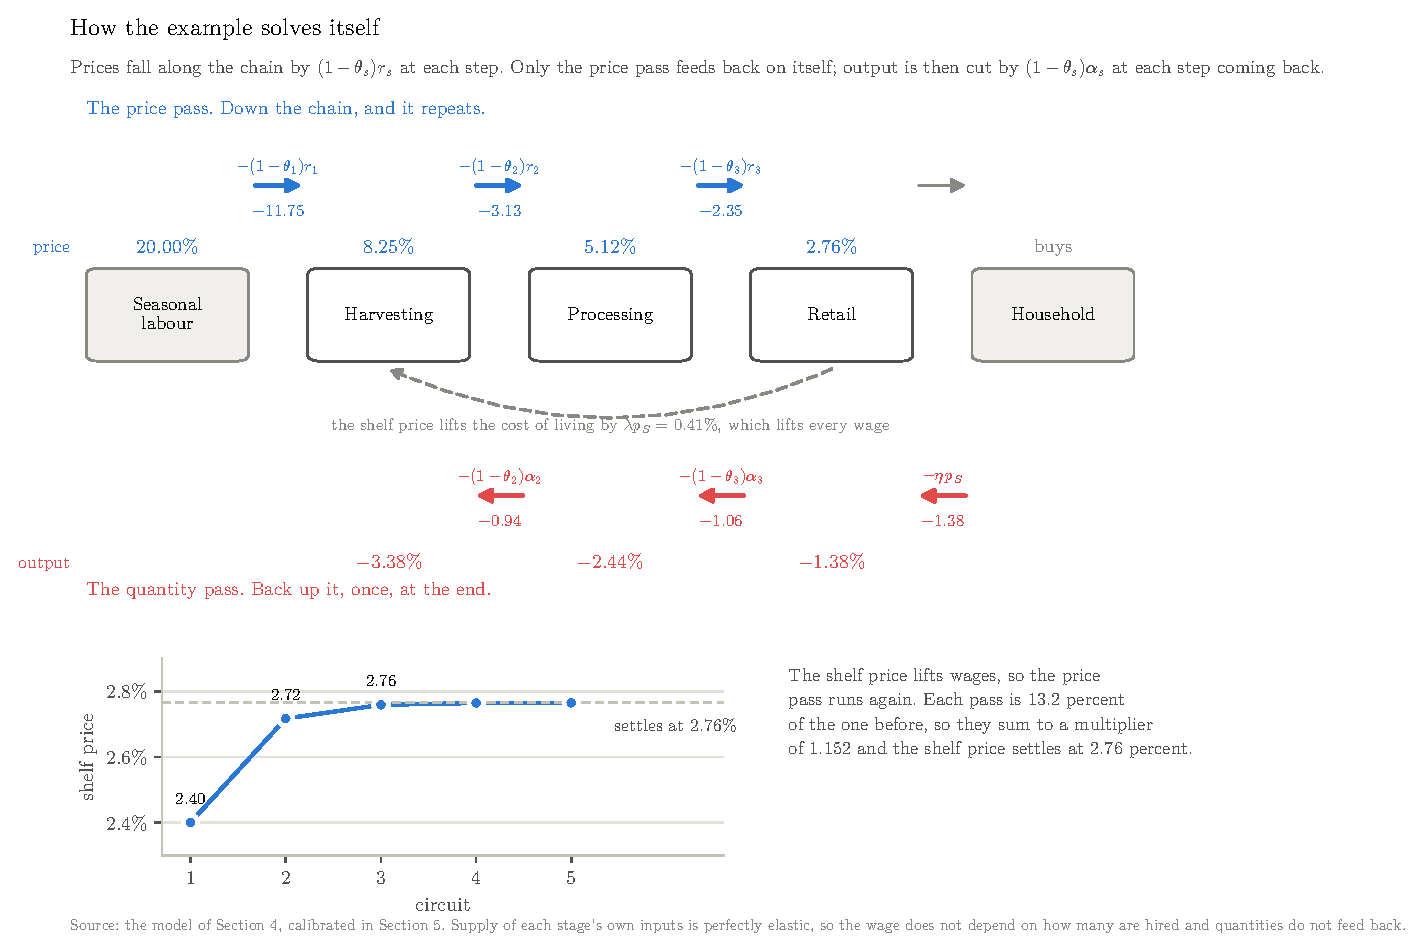
\includegraphics[width=\textwidth]{figures/fig-solve.pdf}
\end{figure}


\section{The Clemens and Lewis example}
\label{sec:example}

Now that the model has been explained, I can apply it to the example of US farming. I assume three producing stages --- harvesting, processing and packing, retail and food service --- and the household. The third stage covers every commercial activity that sells food for consumption: shops, restaurants, canteens, caterers and takeaways. The good is all food, wherever a household buys it.

\begin{table}[htbp]
\centering
\small
\begin{tabularx}{\textwidth}{l l X}
\toprule
\textbf{Parameter} & \textbf{Value} & \textbf{Where it comes from} \\
\midrule
$\Omega$ from 0 to 3 & 0.118 & Measured. This is the value of farm output as a share of household food spending, and the USDA food dollar series reports it: farms received 11.8 cents of every dollar Americans spent on domestically produced food in 2024. \\
$\theta_1$, $\theta_2$, $\theta_3$ & 0.40, 0.60, 0.50 & Chosen to multiply to the measured $\Omega$. The USDA marketing bill divides the other 88 cents between processing, packaging, transport, wholesale and retail, so these three could be measured too. \\
$\sigma_1$, $\sigma_2$, $\sigma_3$ & 0.15, 0.30, 0.45 & Rising downstream. Harvesting is tied to land, season and crop. Processing can change product mix, shorten the season or buy in produce. Retail and food service can change what they stock, though not by much once importing is ruled out: a shop cannot sell more groceries by hiring more staff. On $\sigma_1$: Clemens and Lewis measure 0.8 to 2.2, but that is a firm-level number --- one firm can hire another firm's US workers, while the sector cannot hire its own, and their investment result says equipment and visa labour are used together rather than one instead of the other. So I use a figure well below their range. \\
$\lambda$ & 0.15 & Food at home and at restaurants is about a seventh of total household consumption, which the BLS relative importance weights put at 13.7 percent in December 2024. This restriction moves the price of nothing else, so $\lambda$ is this budget share. \\
$\varepsilon_1$, $\varepsilon_2$, $\varepsilon_3$ & perfectly elastic & Seasonal low-skill work is the kind people move in and out of, so the supply of it to a sector is close to perfectly elastic and the adjustment falls on employment. Section~\ref{sec:range} varies this. \\
$\theta_4$, $\sigma_4$ & 0.15, 0.59 & The household. Food at home and at restaurants takes about a seventh of total household consumption and has few substitutes. The demand elasticity follows from the two: $\eta = \sigma_4(1-\theta_4) = 0.59 \times 0.85 = 0.5$. I set $\sigma_4$ to reach 0.5, so that number is a choice rather than a measurement. Section~\ref{sec:hosp} uses hospitality instead. \\
Rise in $P_X$ & +20\% & A guess, but one that can be re-expressed as a quantity using the demand elasticity of the restricted input. \\
\bottomrule
\end{tabularx}
\end{table}

\subsection{The price at each stage rises}
\label{sec:prices}

\begin{center}
\small
\begin{tabular}{lrrr}
\toprule
 & \textbf{$\Omega$ from 0 to s} & \textbf{weight on the cost of living} & \textbf{Price rise} \\
\midrule
Seasonal labour, $P_X$ & 1.000 & 0.000 & +20.00\% \\
Farm gate, $P_{1}$ & 0.400 & 0.600 & +8.25\% \\
Wholesale packed, $P_{2}$ & 0.240 & 0.760 & +5.12\% \\
Retail shelf, $P_{3}$ & 0.120 & 0.880 & +2.76\% \\
\bottomrule
\end{tabular}
\end{center}

Each price is the cost share times 20 percent, plus one minus the cost share times the 0.41 percent rise in the cost of living. At the farm gate the first dominates. At the shelf the second is most of the weight, but it is multiplied by a very small number.

Seasonal labour is 12 cents of the food dollar. With no indexation at all the shelf price would rise by 2.40 percent, which is 12 percent of 20. With pay indexed to the cost of living it rises by 2.76 percent, which is 13.8 percent of 20. The effective cumulative share is 0.138 against a cost share of 0.120, a ratio of 1.15.

That is a small amplification. Food is about a seventh of total household consumption, so a 2.76 percent rise in its price moves the cost of living by 0.41 percent. Pay indexed to a share that small implies a small wage increase even for a 20 percent input price rise. For an input used throughout the economy, the same mechanism is much larger, which is Section~\ref{sec:everywhere}. That goes to show how important budget shares are, and how important that policies are not devised in isolation of other known (or even known unknown) cost of living changes.

No factor price falls anywhere, but rises are also small. All three rise by 0.41 percent, the rise in the cost of living, because supply is elastic and pay tracks the index. Against selling prices that rise by 8.25, 5.12 and 2.76 percent, that leaves a large gap at every stage, and employment moves instead.

\subsection{Output falls and employment falls at every stage}
\label{sec:empl}

\begin{center}
\small
\setlength{\tabcolsep}{4.2pt}
\begin{tabular}{lrrrrr}
\toprule
 & \multicolumn{1}{c}{Employment} & \multicolumn{2}{c}{Output falls because} & \multicolumn{1}{c}{Output} & \multicolumn{1}{c}{Employment} \\
 & \multicolumn{1}{c}{per unit output} & stages downstream & households & & \\
\midrule
Harvesting & +1.18\% & $-$2.00\% & $-$1.38\% & $-$3.38\% & \textbf{$-$2.21\%} \\
Processing & +1.41\% & $-$1.06\% & $-$1.38\% & $-$2.44\% & \textbf{$-$1.03\%} \\
Retail and food service & +1.06\% & \phantom{$-$}0.00\% & $-$1.38\% & $-$1.38\% & \textbf{$-$0.32\%} \\
\bottomrule
\end{tabular}
\end{center}

The same figures through the recursion, which shows what each stage does rather than what happens to it:

\begin{center}
\small
\begin{tabular}{lrrrr}
\toprule
 & Cost share & Shift in input mix & Kept by the stage & Employment \\
 & $\theta_s$ & $\alpha_s$ & $\theta_s \alpha_s$ & $l_s$ \\
\midrule
Harvesting & 0.40 & +2.94\% & +1.18\% & \textbf{$-$2.21\%} \\
Processing & 0.60 & +2.35\% & +1.41\% & \textbf{$-$1.03\%} \\
Retail and food service & 0.50 & +2.12\% & +1.06\% & \textbf{$-$0.32\%} \\
Household & 0.15 & +1.63\% & +0.24\% & \textbf{+0.24\%}$^{*}$ \\
\bottomrule
\end{tabular}

\smallskip
\begin{minipage}{0.9\textwidth}
\footnotesize $^{*}$ In this case, the household is not a firm and does not employ anyone. Its entry is $l_4$, the change in what it spends on everything other than this good, which is what the recursion needs to start.
\end{minipage}
\end{center}

We work up the rows from the bottom. The household shifts its mix by 1.63 percent and keeps 0.15 $\times$ 1.63 = 0.24 percent of that as extra spending on everything else. Retail then gets 0.24 + 1.06 $-$ 1.63 = $-$0.32 percent: it keeps 1.06 of its own shift and loses the household's whole 1.63. Processing gets $-$0.32 + 1.41 $-$ 2.12 = $-$1.03 percent, losing retail's whole 2.12. Harvesting gets $-$1.03 + 1.18 $-$ 2.35 = $-$2.21 percent, losing processing's whole 2.35.

We can read the rows across. Each stage employs more per unit of output, between 1.06 and 1.41 percent more. At every stage output falls by more than that, so employment falls at all three.

The household column is one number. Households buy 1.38 percent less, so output falls 1.38 percent at every stage on that account. No firm's decisions change it.

The other two columns are where the stages differ. Harvesting's output falls a further 2.00 percent because processing and retail buy less per unit of their own output. Processing's falls a further 1.06 percent because retail does. Retail's does not fall at all on this account, because no producing stage buys from it.

\textbf{The conclusions on retail are the most sensitive.} The closed form in equation~(\ref{eq:lastst}) says the last stage loses employment only while $\sigma_3 < \sigma_4$. Here that is 0.45 against 0.59, so retail loses, but not by much: 0.32 percent. Push $\sigma_3$ above 0.59 --- which is what you would get if a supermarket could switch to imported food or any other unrestricted input, the thing this model rules out --- and retail gains jobs instead.

\subsection{Hospitality}
\label{sec:hosp}

Not every H-2B chain ends at a supermarket. Hospitality, amusement and golf together are a sizeable part of the programme. Households substitute away from those services more readily, and they take a twentieth of total household consumption rather than a seventh, so $\eta$ = 1.5 and $\lambda$ = 0.05.

Employment falls by 4.60, 3.41 and 2.69 percent, and the shelf price rises 2.51 percent. The losses are larger at every stage and the gap between stages is smaller, because the household term is larger and the same at each of them.

\subsection{How much of this holds over a range}
\label{sec:range}

Lowering $\varepsilon$ moves the adjustment from jobs to pay, and cannot change the sign of either.

\begin{center}
\small
\begin{tabular}{lrrr}
\toprule
$\varepsilon$ at every stage & Shelf price & Factor prices & Employment \\
\midrule
perfectly elastic & +2.76\% & +0.41, +0.41, +0.41 & $-$2.21, $-$1.03, $-$0.32 \\
5 & +2.60\% & $-$0.02, +0.21, +0.33 & $-$2.06, $-$0.92, $-$0.28 \\
2 & +2.41\% & $-$0.57, $-$0.04, +0.25 & $-$1.87, $-$0.80, $-$0.23 \\
1 & +2.18\% & $-$1.30, $-$0.32, +0.15 & $-$1.63, $-$0.64, $-$0.18 \\
0.5 & +1.88\% & $-$2.31, $-$0.64, +0.05 & $-$1.30, $-$0.46, $-$0.12 \\
0.2 & +1.49\% & $-$3.83, $-$0.97, $-$0.05 & $-$0.81, $-$0.24, $-$0.05 \\
0 (supply fixed) & +0.95\% & $-$6.46, $-$1.16, $-$0.11 & 0, 0, 0 \\
\bottomrule
\end{tabular}
\end{center}

At the bottom row nobody loses a job and harvesting takes a 6.46 percent pay cut instead. Harvesting loses in all cases. At the top row it loses 2.21 percent of its jobs, at the bottom row it keeps them all and loses 6.46 percent of its pay. Between the two ends the loss is shared, and the total loss is largest at the top: the shelf price rises most, so households buy least, when pay is defended.

\section{When the input is used everywhere}
\label{sec:everywhere}

Everything above has $\lambda$ = 0.15, because this restriction moves the price of food and nothing else. Raise $\lambda$ and the same mechanism is a macroeconomic event.

\begin{center}
\small
\begin{tabular}{lrrrr}
\toprule
$\lambda$ & Effective share & Shelf price & Cost of living & Employment \\
\midrule
0 (pay not indexed) & 0.120 & +2.40\% & 0.00\% & $-$2.04, $-$0.84, $-$0.12 \\
0.15 (food alone) & 0.138 & +2.76\% & +0.41\% & $-$2.21, $-$1.03, $-$0.32 \\
0.30 & 0.163 & +3.26\% & +0.98\% & $-$2.43, $-$1.29, $-$0.60 \\
0.50 & 0.214 & +4.29\% & +2.14\% & $-$2.89, $-$1.82, $-$1.18 \\
0.70 & 0.313 & +6.25\% & +4.38\% & $-$3.78, $-$2.84, $-$2.28 \\
0.90 & 0.577 & +11.54\% & +10.38\% & $-$6.17, $-$5.60, $-$5.25 \\
\bottomrule
\end{tabular}
\end{center}

At $\lambda$ = 0.9 a 20 percent rise in one input's price raises the shelf price by 11.5 percent, raises the cost of living by 10.4, and costs every stage between 5.3 and 6.2 percent of its employment. The effective share is 0.577 against a cost share of 0.120: the input matters five times its weight in costs.

This result is explained by two things. Pay indexed to an index that is itself rising feeds back into costs, which raises the index again. And as $\lambda$ rises the stages become alike, because the household term grows and the terms that differ between stages shrink. At $\lambda$ = 0.9 the spread across the three stages is 0.9 points; at $\lambda$ = 0.15 it is 1.9.

This is oil, and it is what Michael Bruno and Jeffrey Sachs called real wage resistance in 1985, when they explained why the oil shocks of the 1970s led to much higher unemployment in some economies than in others, and attributed the difference to how far real wages adjusted. Energy is about 6 percent of American household consumption and an input to most of the rest, so its $\lambda$ is far above its direct weight. Tariffs on inputs used everywhere belong in the same group. What this shows is that the risk of wage resistance is real.

\section{Objections}
\label{sec:obj}

I take these from what is argued in public. Some would change the policy conclusion if the facts went their way. But thinking about those facts is itself disciplining.

\subsection{It is the employer that sets the wage}

The objection. An H-2B worker cannot change employer without losing the right to work. So the employer sets the wage rather than the market, and it is below the revenue the last worker brings in, as in a monopsonistic labour market. A constraint on the employer can then raise pay without cutting employment, in the same way a minimum wage can where one buyer faces many sellers of labour. A cap on visas is one such constraint.

My answer. We first need to be sure that these markets are monopsonistic. One piece of evidence we would need to see is that firms hold abnormal profit at the stage where the input is restricted. My chain assumes abnormal profit is zero or constant, so I have assumed that surplus away rather than shown it is absent. Another interesting area to investigate is the mobility of workers and tasks that can be unbundled. But if markets were monopsonistic and if nothing could be done about that, it might make a difference and the model should be extended or changed.


\subsection{Negative externalities and repugnant features}

The objection. Some inputs have negative externalities and unacceptable features or ``bads'': fossil fuels, congested roads, labour working in conditions we would not accept for ourselves. Shrinking an industry that runs on such an input could raise welfare even though output and employment fall.

My answer. That could of course be valid. What my figures supply is the size of the loss, and what that depends on. Too often, that is not mentioned in the debate. Yes, some industries are so repugnant that we would want to ignore the employment and income costs of shutting them down. But I think we should be careful not to overuse that argument to where we cannot afford it. After all, in times of economic distress, governments have ended the prohibition of banned items in an effort to stimulate the economy and had to become more pragmatic.

In this case, the public should be aware that any negative externality removed from using seasonal farm labour could imply a 2.21 percent fall in employment at harvesting and possibly shrink the industry.

\subsection{Wages divide a surplus and do not measure a product}

The objection. Marginal products are the wrong way of doing this. Pay is a share of a surplus, settled by bargaining power. Restrict labour supply and the workers' share rises and the owners' share falls. Employment need not move, because firms have margins to absorb the change.

My answer. The objection treats restricting migrant labour as restricting all labour. It is not. It removes something the remaining workers work alongside, so their marginal product can fall rather than rise, and with it, either their pay or their employment chances. The model says which: with supply perfectly elastic harvesting loses 2.21 percent of its jobs, and with supply fixed it keeps them all and takes a 6.46 percent pay cut. Neither is a share moving towards workers.

I cannot settle the question inside the model, because zero abnormal profit assumes away the surplus the objection is about. Yet if that were true, the pay and employment of the workers already here should rise where migrant hiring was cut. Clemens and Lewis found that employment of low-skill American workers at the losing firms did not rise, and in the rural sample they specified in advance the two moved together, at 0.61.

A model built on marginal products cannot refute a world view built on bargaining. What I think would help push the two world views together is a measurement of how far pay at each stage follows the cost of living, and of how elastic the supply of workers to each stage is.

\subsection{Restrict them and they will invest instead}

The objection. Employers use the programme because it is cheaper than paying more or buying machinery. If you remove access to cheap labour then they will invest. This is the most common objection in public.

I would categorise this alongside other market-failure arguments, though the failure here is in credit: cheap labour lets a farmer postpone an investment that a bank will not finance. That said, in the public mind's eye, capital intensive production is often better, more high growth, more complementary to skilled labour and environmentally cleaner.

Whether removing the cheap labour brings the investment forward is an old question. Habakkuk argued in 1962 that American labour scarcity is why America mechanised faster than Britain. Acemoglu settled the condition under which that works: labour scarcity encourages new technology only where the technology is strongly labour saving, meaning it reduces what the last worker adds. Where technology is labour complementary, scarcity discourages it, and he notes that the complementary case is what most standard growth models assume. Clemens, Lewis and Postel tested it on exactly this policy. When the United States excluded Mexican bracero workers in 1964, farms growing tomatoes, cotton and sugar beets mechanised quickly, because the machines already existed and could be put to work without large fixed costs. Farms growing asparagus, strawberries, lettuce and melons had no such choice, and simply grew less.

I would only note that Clemens and Lewis found that at the firms that could hire the workers they asked for, investment in equipment, vehicles and buildings rose with an elasticity between 1.5 and 2.1. Equipment and visa labour are used more together rather than one instead of the other, so restricting the labour reduced the investment. This again calls for a case by case analysis.

\subsection{Other caveats}
\label{sec:caveats}

To be fair to Clemens and Lewis, their experiment was at a firm by firm level, whereas my model restricts a sector. A single firm cannot raise its price, and its customers buy from a rival that won its draw. The experiment does not test what I have modelled.

On the employment of American workers, I said above that native hiring did not rise and may have fallen slightly.  Clemens and Lewis estimate how American employment moves with H-2B employment at $+0.10$, which is not statistically different from zero. Losing the draw cut H-2B employment by about half, a fall of 0.62 in natural logs. Multiplying the two gives 0.062, a fall of about 6 percent in American employment. Zero is still inside the range, and so is a fall of that magnitude.

The chain is not the chain the experiment studied either. H-2B is non-agricultural, and in the authors' survey the largest group of requested workers is groundskeeping and outdoor maintenance, between 36 and 46 percent depending on which version of their paper you read. Seafood processing, the part of the programme that does run through a food chain, is 6 to 10 percent. I use food because the cost shares along it are measured and published. The mechanism is general. The calibration illustrates it and does not model the programme.

The result does depend especially on two of my chosen parameter values. At the top of the chain, harvesting loses employment only while $\sigma_1$ stays low enough that shifting its input mix does not outweigh its falling output; I use 0.15 against the 0.8 to 2.2 that Clemens and Lewis measure at firm level, for the reason given in Section~\ref{sec:example}. At the bottom, retail keeps losing employment only while $\sigma_3$ stays below $\sigma_4$, 0.45 against 0.59. Both numbers are argued rather than estimated, and the sign at each end of the chain turns on them.

In principle the substitution elasticities $\sigma_s$ have no upper bound. They can be any non-negative number: zero is fixed input proportions, one is Cobb-Douglas, and large values are close substitutes. For example $\sigma_s$ might have to adjust where imported alternatives were easily accessible. Policy people call that leakage. A crab processor that can buy imported crab meat has a high $\sigma_2$ and loses less employment, and the fall moves further upstream to the domestic harvesters. The same policy reduces employment for different workers depending on whether the intermediate input can be imported, and I have not measured which.

As I note in Section~\ref{sec:ignore}, the 11.8 cents may not be the correct value. It is the cost share of all farm value in the food dollar, and hired seasonal labour is a minority of farm cash costs. For visa labour alone the cumulative share is perhaps 0.01 to 0.03, and all three terms fall with it.

A visa cap restricts a quantity, not a price, and my 20 percent could be off. The model does map one to the other: on this calibration the demand for seasonal labour has an elasticity of 0.26, so a 20 percent rise in its price is a 5.1 percent cut in the quantity of it. Read the other way, a 10 percent cut needs a 39 percent price rise.

$\lambda$ is not a published figure. It is the share of the consumer basket whose price moves, direct and indirect, so the direct budget share is a floor on it and a full estimate needs an input-output calculation. For food the two are close. For energy they are not.

The model has one period, so there is no storage and no forward or futures market. Every stage buys the input and uses it in the same period. No stage holds any back for later, and no stage fixes a price in advance.

That suits seasonal labour, which cannot be stored: a day of harvesting not done in August cannot be done in December. It suits other restricted inputs less well. A buyer who holds stock, or who bought forward before the restriction, can spread a temporary shortage over months, so the fall in employment would be smaller in any one quarter and longer in total. Williams and Wright set out how storage and futures prices work together, and downstream buyers do use both. For an input drawn from a finite stock, a restriction today also moves the price expected tomorrow, which is Hotelling's result from 1931. This matters most where I extend the argument: Section~\ref{sec:everywhere} raises $\lambda$ and calls the result oil, and oil is stored and traded forward.

The household keeps its total spending fixed and changes only what it spends the money on. A household facing higher prices may save more and spend less in total, and output would then fall at every stage by more than the figures here. Here, these are jobs lost in one chain and not employment in the whole economy.

\subsection{Reproducing the numbers}

Every figure in this note is solved in code. The model is about a hundred lines of Python and needs numpy alone. A second script recomputes all 66 printed figures and checks each against the value in the text, and it reports a failure if any of them moves. Both are archived with this note at DOI \href{https://doi.org/10.5281/zenodo.22836881}{10.5281/zenodo.22836881}.

Four structural claims were also checked against a direct solution of the whole system over randomly drawn chains with $S$ from 1 to 6 and every parameter drawn at random: the matrix of Section~\ref{sec:solving} over 20,000 chains, agreeing to $2.0 \times 10^{-15}$; the recovery equations over 3,000, to $5.6 \times 10^{-16}$; the employment recursion over 20,000, to $3.3 \times 10^{-16}$; and the last-stage closed form over 5,000, to $1.7 \times 10^{-16}$.

\section{Conclusion}
\label{sec:conc}

Alfred Marshall set out indirect demand in 1890. ``The demand for raw materials and other means of production,'' he wrote, ``is indirect and is derived from the direct demand for those directly serviceable products which they help to produce.'' His example was building: ``the direct demand for houses gives rise to a joint demand for the labour of all the various building trades, and for bricks, stone, wood, etc.''

Production chains are longer now than the building trades he described, and policy restricts the first link more often: visas, tariffs, export licences, permits.

Restrict the supply of an input at the top of a chain and it is possible that employment falls at every stage of it. It falls because output falls, and output falls by more than employment per unit of output rises.

In percentage terms, employment falls most at the stage nearest the restriction. That stage can change its input mix least, and most of what it produces is bought by firms that are buying less. On these figures harvesting loses 2.21 percent of its employment and retail, two stages away, loses 0.32 percent, about seven times less.

These are percentages of each stage's own employment. The model has no employment levels in it, so it does not say which stage loses the greater number of workers. A stage with a smaller percentage loss and many more workers can lose more of them: on these figures retail and food service would do so once it employs more than 6.79 times as many people as harvesting.

The final stages can, in principle, grow. It depends on whether they can switch out of the restricted chain more than their customers switch away from them entirely. That is I think a good description of how product-led businesses work; they keep their attention on both the consumer switching and technology feasibility and try to keep the product ahead of the market, or influence the market.


Making pay compensate for the cost of living can make things worse, by feeding the price rise back into costs. For food price rises, that is a small effect: the share of the original rise reaching the shelf rises from 12 percent to 13.8, and makes households buy 1.38 percent less rather than 1.20. For an input used throughout the economy the impact is serious, taking the same share to 58 percent and costing every stage over five percent of its employment. This is a reminder of how employment and pay are connected.

In this case, the cap was set to protect American jobs and pay. Yet, it may be that employment falls at every stage of the chain, that the largest fall (in percentage terms) is at the stage where the cap applies, and that pay rises by less than selling prices everywhere. 

Governments cannot protect us from all costs and we need to engage more in the political economic debate beyond the clamour to do something. Voters should recognise the limits of governments and policy institutions and be careful what they ask for.  This may not just apply to restrictions on immigration. It may apply to a tariff on imported steel, a licence for rare earths, and so on.

\section*{References}
Acemoglu, D. (2010). ``When Does Labor Scarcity Encourage Innovation?'' \emph{Journal of Political Economy}, 118(6), 1037--1078.

Bruno, M., and Sachs, J. D. (1985). \emph{Economics of Worldwide Stagflation}. Harvard University Press.

Clemens, M. A., Lewis, E. G., and Postel, H. M. (2018). ``Immigration Restrictions as Active Labor Market Policy: Evidence from the Mexican \emph{Bracero} Exclusion.'' \emph{American Economic Review}, 108(6), 1468--1487.

Clemens, M. A., and Lewis, E. G. (2026). ``The Effect of Low-Skill Immigration Restrictions on US Firms and Workers: Evidence from a Randomized Lottery.'' \emph{American Economic Journal: Applied Economics}, 18(3), 43--82. \href{https://doi.org/10.1257/app.20250049}{doi:10.1257/app.20250049}. Working paper version: NBER Working Paper 30589. Summary at \href{https://www.aeaweb.org/research/immigration-restrictions-firms-workers}{aeaweb.org}.

Habakkuk, H. J. (1962). \emph{American and British Technology in the Nineteenth Century: The Search for Labour-Saving Inventions}. Cambridge University Press.

de Haas, H. (2023). \emph{How Migration Really Works: 22 Things You Need to Know about the Most Divisive Issue in Politics}. Penguin.

Hotelling, H. (1931). ``The Economics of Exhaustible Resources.'' \emph{Journal of Political Economy}, 39(2), 137--175.

Kremer, M. (1993). ``The O-Ring Theory of Economic Development.'' \emph{Quarterly Journal of Economics}, 108(3), 551--575.

Marshall, A. (1890). \emph{Principles of Economics}. Macmillan. Book V, Chapter VI, ``Joint and Composite Demand. Joint and Composite Supply.''

Rittel, H. W. J., and Webber, M. M. (1973). ``Dilemmas in a General Theory of
Planning.'' \emph{Policy Sciences}, 4(2), 155--169.

Williams, J. C., and Wright, B. D. (1991). \emph{Storage and Commodity Markets}. Cambridge University Press.

US Department of Agriculture, Economic Research Service. \href{https://www.ers.usda.gov/data-products/charts-of-note/114074}{Food Dollar Series: farms received 11.8 cents per dollar spent on domestically produced food in 2024}.

\end{document}
